\documentclass{standalone}
\usepackage{tikz}
\begin{document}
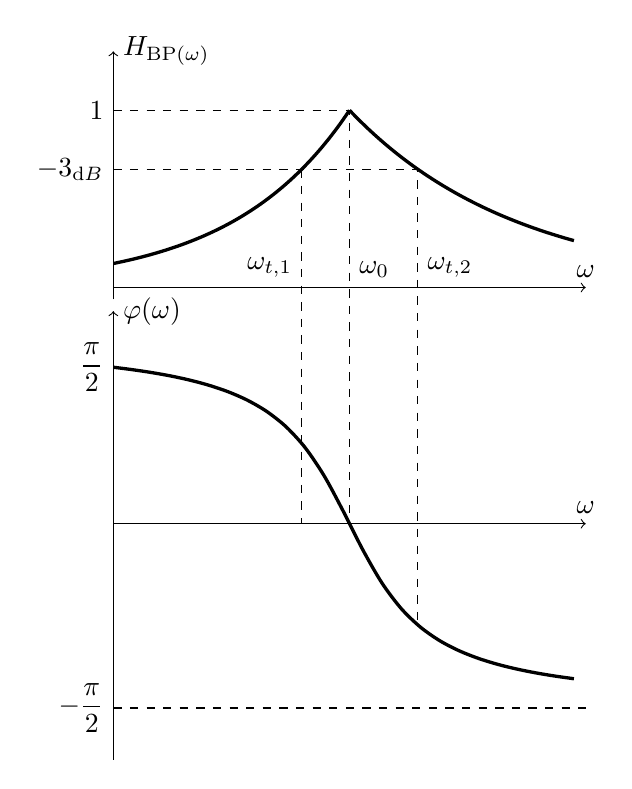
\begin{tikzpicture}[scale=1.5]
    \draw[->](0,1.9)--(0,4)node[right]{$H_{\mathrm{BP}(\omega)}$};
    \draw[->](0,2)--(4,2)node[above]{$\omega$};
    \draw[very thick,smooth, domain=0:2]plot(\x,{1.5*e^(\x-2)+2});
    \draw[very thick,smooth, domain=2:3.9]plot(\x,{1.5*e^(0.7*(-\x+2))+2});
    \draw[->](0,-2)--(0,1.8)node[right]{$\varphi(\omega)$};
    \draw[->](0,0)--(4,0)node[above]{$\omega$};
    \draw[very thick, smooth, domain=0:3.9]plot(\x,{pi/180*atan(-2*\x+4)});
    \draw[dashed](0,3.5)node[left]{$1$}--(2,3.5)--(2,2)node[above right]{$\omega_0$}--(2,0);
    \node[left]at(0,1.326){$\displaystyle\frac{\pi}{2}$};
    \draw[dashed](0,-1.56)node[left]{$-\displaystyle\frac{\pi}{2}$}--(4,-1.56);
    \draw[dashed](0,3)node[left]{$-3_{\mathrm{d}B}$}--(1.595,3)--(2.579,3)--(2.579,2)node[above right]{$\omega_{t,2}$}--(2.579,-0.858);
    \draw[dashed](1.595,3)--(1.595,2)node[above left]{$\omega_{t,1}$}--(1.595,0);
\end{tikzpicture}
\end{document}